\begin{figure}[h]
	\scalebox{0.75}	{
		\centering
		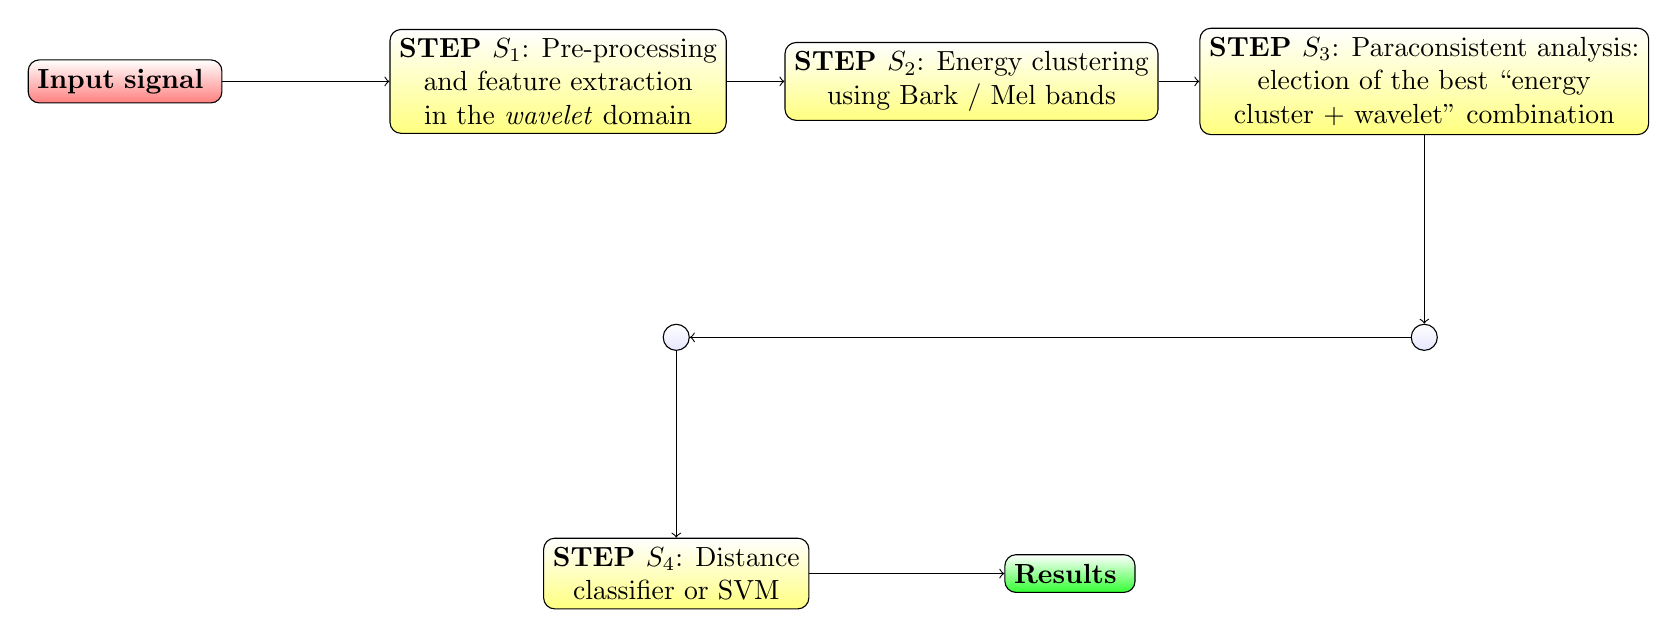
\begin{tikzpicture} 
			\node (z1)[shape=rectangle, rounded corners, draw, align=center, top color=white, bottom color=red!50] 
			at (0,2){
				\textbf{Input} \textbf{signal}
			}; 
				
			\node (z2)[shape=rectangle, rounded corners, draw, align=center, top color=white, bottom color=yellow!50] 
			at (5.5,2){
				\textbf{STEP $S_1$}: Pre-processing \\
				and feature extraction \\
				in the \textit{wavelet} domain 
			}; 	
			
			\node (z3)[shape=rectangle, rounded corners, draw, align=center, top color=white, bottom color=yellow!50] 
			at (10.75,2){
				\textbf{STEP $S_2$}: Energy clustering \\
				using Bark / Mel bands 
			}; 	
			
			\node (z4)[shape=rectangle, rounded corners, draw, align=center, top color=white, bottom color=yellow!50] 
			at (16.5,2){
				\textbf{STEP $S_3$}: Paraconsistent 
				analysis: \\ election of the best 
				``energy \\ cluster + wavelet'' combination 
			}; 
			
			\node (z5)[shape=circle, draw, align=center, top color=white, bottom color=blue!10] 
			at (16.5,-1.25){}; 
					
			\node (z6)[shape=circle, draw, align=center, top color=white, bottom color=blue!10] 
			at (7,-1.25) {};
			
			\node (z7)[shape=rectangle, rounded corners, draw, align=center, top color=white, bottom color=yellow!50] 
			at (7,-4.25) {
				\textbf{STEP $S_4$}: Distance \\ classifier or SVM
			};
			
			\node (z8)[shape=rectangle, rounded corners, draw, align=center, top color=white, bottom color=green!80] 
			at (12,-4.25) {
				\textbf{Results}
			};
			
			\path[->] (z1) edge (z2);
			\path[->] (z2) edge (z3);
			\path[->] (z3) edge (z4);
			\path[->] (z4) edge (z5);
			\path[->] (z5) edge (z6);
			\path[->] (z6) edge (z7);	
			\path[->] (z7) edge (z8);
		\end{tikzpicture}
	}
	\caption{Proposed approach structure}
	\label{fig:propApproachStruct}
\end{figure}